% This is a sample LaTeX input file.  (Version of 12 August 2004.)
%
% A '%' character causes TeX to ignore all remaining text on the line,
% and is used for comments like this one.
\documentclass[twocolumn]{article}      % Specifies the document class
\usepackage{authblk}
\usepackage{amsmath}
\usepackage{algorithm}
\usepackage{algpseudocode}
\usepackage{graphicx}
\usepackage{ragged2e}
\usepackage{tabu}
\newcommand\NoDo{\renewcommand\algorithmicdo{}}
\newcommand\ReDo{\renewcommand\algorithmicdo{\textbf{do}}}
\newcommand\NoThen{\renewcommand\algorithmicthen{}}
\newcommand\ReThen{\renewcommand\algorithmicthen{\textbf{then}}}
\renewcommand\algorithmicthen{}
\renewcommand\algorithmicdo{}
\makeatletter
\def\BState{\State\hskip-\ALG@thistlm}
\makeatother
                             % The preamble begins here.
\title{Computing the reciprocal (Multiplicative inverse) of any given number}  % Declares the document's title.
 \author{Akshay Gupta~{IIT2017505}, \hspace{6pt}Naman Deept~{IIT2017507}  \\Dept. of Information Technology\\Indian Institute of Information Technology  Allahabad
 }
 
%\date{\today}      % Deleting this command produces today's date.
\renewcommand\Authands{ and }
\newcommand{\ip}[2]{(#1, #2)}
                             % Defines \ip{arg1}{arg2} to mean
                             % (arg1, arg2).

%\newcommand{\ip}[2]{\langle #1 | #2\rangle}
                             % This is an alternative definition of
                             % \ip that is commented out.

\begin{document}             % End of preamble and beginning of text.
\begin{titlepage}

\newcommand{\HRule}{\rule{\linewidth}{0.5mm}} % Defines a new command for the horizontal lines, change thickness here

\center % Center everything on the page
 
%----------------------------------------------------------------------------------------
%	HEADING SECTIONS
%----------------------------------------------------------------------------------------

\textsc{\LARGE Assignment 2}\\[1.5cm] % Name of your university/college
\includegraphics[scale=0.7]{iiitlogo2.jpg}\\[1cm]
\textsc{\Large Design and Analysis of Algorithm}\\[0.5cm] % Major heading such as course name
\textsc{\large IDAA432C}\\[0.5cm] % Minor heading such as course title

%----------------------------------------------------------------------------------------
%	TITLE SECTION
%----------------------------------------------------------------------------------------

\HRule \\[0.4cm]
{ \large \bfseries To Find the reciprocal of a given Number without using Multiplication, Division and Modulus Operator }\\[0.4cm] % Title of your document
\HRule \\[1.5cm]
 
%----------------------------------------------------------------------------------------
%	AUTHOR SECTION
%----------------------------------------------------------------------------------------

\begin{minipage}{0.4\textwidth}
\begin{flushleft} \large
\textbf{\emph{Submitted By:}}\\
Akshay Gupta \textbf{(IIT2017505)}\\
Naman Deept \textbf{(IIT2017507)}
\end{flushleft}
\end{minipage}\\[2cm]

% If you don't want a supervisor, uncomment the two lines below and remove the section above
%\Large \emph{Author:}\\
%John \textsc{Smith}\\[3cm] % Your name

%----------------------------------------------------------------------------------------
%	DATE SECTION
%----------------------------------------------------------------------------------------

{\large \today}\\[2cm] % Date, change the \today to a set date if you want to be precise

\vfill % Fill the rest of the page with whitespace

\end{titlepage}
\maketitle                   % Produces the title.


    % Produces section heading.  Lower-level
                             % sections are begun with similar 
                             % \subsection and \subsubsection commands.

\section{Abstract} 
This paper introduces an efficient algorithm for any integer ,to find the reciprocal of the number and then goes on to find the reciprocal of any real number to a required precision without using multiplication , division or modulus operator.\\
\textbf{Keywords}: \textit{Multiplicative Inverse}, \textit{Reciprocal}, \textit{Inverse}, \textit{Newton Raphson}, \textit{Bit Manipulation}
\section{Introduction}
In mathematics, a multiplicative inverse or reciprocal for a number $x$, denoted by $1/x$ or ${x^{-1}}$, is a number which when multiplied by $x$ yields the multiplicative identity, $1$. The multiplicative inverse of a fraction $a/b$ is $b/a$. For the multiplicative inverse of a real number, divide 1 by the number. For example, the reciprocal of $5$ is one fifth ($1/5$ or $0.2$), and the reciprocal of $0.25$ is $1$ divided by $0.25$, or $4$. The reciprocal function, the function $f(x)$ that maps $x$ to $1/x$, is one of the simplest examples of a function which is its own inverse (an involution).\\
To find the reciprocal of a given number without using multiplication , division and modulus operators we can either use either bit manipulation , iterative subtraction or Newton-Raphson method.
\section{Proposed Method}
\textbf{Input} : Given any number,to find the multiplicative inverse of the number to any given precision using various approaches.The number can be any number integer and any rational number.
\subsection{Bit Manipulation}
The algorithm of Bit Manipulation can be able to compute only those multiplicative inverses where the value of the desired number is only an integer. 
\subsubsection{Algorithm}
\begin{algorithm}
\begin{algorithmic}[1]
\Procedure{dividemod}{$dividend,num$}
\State $quotient \gets 0$
\State $temp \gets 0$
\For{$i \gets 31\hspace{2pt} to\hspace{2pt} 0$}
\If{$temp + (divisor<<i) \leq 1$}
\State $temp \gets temp +divisor <<1$
\State $ quotient \gets quotient | 1<<i$
\State $quotientresult \gets quotient$
\EndIf
\EndFor
\State return divisionresult ,quotientresult
\EndProcedure
\end{algorithmic}
\end{algorithm}
\begin{algorithm}
\begin{algorithmic}[1]
\Procedure{divide}{$dividend,num$}
\State $NoDecimal \gets 1$
\State $quotient \gets divisionresult$
\State $dividend \gets quotientresult$
\If{$dividend !=0$}
\State $quotient \gets quotient+"."$
\EndIf
\While{$NoDecimal \leq 10$ and $dividend \neq 0$}
\State $dividend$ $\gets$ dividend$<<$3 + dividend$<<$1
\State $dividemod(dividend,divisor)$
\State $quotient \gets quotient + quotientresult$
\State $dividend \gets dividendresult$
\State $NoDecimal \gets NoDecimal +1$
\EndWhile
\State return quotient
\EndProcedure
\end{algorithmic}
\end{algorithm}
\begin{algorithm}
\end{algorithm}
\subsubsection{Time Complexity Analysis}
\textbf{Best Case}- Given algorithm in the best case scenario works on $\Omega($log(n)$)$.These are those numbers who divide numbers which are power of 10 perfectly.\\
\textbf{Worst Case}- Given algorithm in the worst case scenario will be proportional to $O(log(n)\times{b})$.Which will be very large if non - terminating , non -repeating number decimal producing or repeating decimals point generating numbers are there.Where $b$ is the desired precision level. 
\subsection{Iterative Subtraction}
This method works for all real number $n$ . Here first for any desired precision, given number is first converted to a corresponding integer and then smallest power of 10 larger than the corresponding integer is subtracted from it to generate the quotient . The same procedure is done via iteration to generate till the desired precision and then added to quotient through string manipulation .
\newpage
\begin{algorithm}
\begin{algorithmic}
\Procedure{generateZero}{num}
\State $temp$ $\gets$ $emptyString$
\State $numZero$ $\gets$ $EmptyString$
\State $temp$ $\gets$ $num$ ToString
\For {$i$ $\gets$ $1$\hspace{2pt} to\hspace{2pt} $length(temp)$}
\If{$temp.charAt(i)$ $equals$ '.'}
\State continue
\State $numZero$ $\gets$ $numZero$ $+$ $'0'$
\EndIf
\EndFor
\State return $numZero$
\end{algorithmic}
\end{algorithm}
\begin{algorithm}
\begin{algorithmic}
\Procedure{addZero}{num}
\State $Result$ $\gets$ $emptyString$
\For{$i$ $\gets$ $1$\hspace{2pt} to\hspace{2pt} $num$}
\State $Result$ $\gets$ $Result$ $+$ $0$
\EndFor
\State return $Result$
\end{algorithmic}
\end{algorithm}
\begin{algorithm}
\begin{algorithmic}
\Procedure{returnback}{num}
\State $str$ $\gets$ $emptyString$
\State $res$ $\gets$ $emptyString$
\State $str$ $\gets$ $num$ ToString
\For {$i$ $\gets$ $1$\hspace{2pt} to\hspace{2pt} $length(str)$}
\If{$temp.charAt(i)$ $equals$ '.'}
\State continue
\State $res$ $\gets$ $res$ $+$ $str.charAt(i)$
\EndIf
\EndFor
\State return $res$ To Integer
\end{algorithmic}
\end{algorithm}
\begin{algorithm}
\begin{algorithmic}[1]
\Procedure{findreciprocal}{$num$}
\State  Result $\gets$ \textit{Empty String}
\If{$num$ $<$ $0$}
\State Result $\gets$ $"-0."$
\EndIf
\If{$num$ $<$ $0$ and $num$ notEquals $1$}
\State Result $\gets$ $"0."$ 
\State $num$ $\gets$ $-num$
\EndIf
\If{$num$ equals $1$}
\State Result $\gets$ Empty String
\EndIf
\State $string$  $\gets$ ${Empty String}$
\State $Zeroes$  $\gets$ ${Empty String}$
\State $string$ $\gets$  ${num(To String)}$
\State $Zeroes$ $\gets$ $1$ + ${GenerateZeroes(num)}$
\State $Dividend$ $\gets$ $0$
\State $Divisor$ $\gets$ $0$
\State $Dividend$ $\gets$ $Zeroes$ (To Integer)
\State $Divisor$ $\gets$ $Returnback(num)$
\State $Precision$ $\gets$ $0$
\State $Quotient$ $\gets$ $0$
\State $Result$ $\gets$ Result $+$ $generateAZero(num)$
\While ${Precision \leq 10}$  
\State $Quotient$ $\gets$ $0$
\While $Dividend$ $\geq$ $Divisor$
\State $Dividend$ $\gets$ $Dividend$ $-$ $Divisor$ 
\State $Quotient$ $\gets$ $Quotient$ $+$ $1$
\EndWhile
\If{$Dividend$ $equals$ $0$}
\State $Break$
\EndIf
\State $DividendString$ $\gets$ $EmptyString$
\State $DividendString$ $\gets$ $Dividend$ ToString
\State $Counter$ $\gets$ $0$
\While $true$
\State $Dividend$ $\gets$ $DividendString$ ToInt
\State $DividendStr$ $\gets$ $DividendStr$ + $"0"$
\If{$Dividend$ $>$ $Divisor$}
\State Break
\EndIf
\State $Precision$ $\gets$ $Precision$ $+$ $1$
\State $Counter$ $\gets$ $Counter$ $+$ $1$
\EndWhile
\State $Result$ $\gets$ $Result$ $+$ $addZero(Counter)$
\State $Precision$ $\gets$ $Precision$ $+$ $1$
\State $Result$ $\gets$ Result $+$ $Quotient$ 
\EndWhile
\State return $Result$
\EndProcedure
\end{algorithmic}
\end{algorithm}
\subsubsection{Time Complexity Analysis}
\paragraph{Best Case Analysis} : The best case for the Iterative Subtraction holds when the numbers are  perfect powers of 2 or 5 or both. i.e of the form $2^n$ ,$5^n$ or $10^n$. When we consider the analysis for this case, we observe that for the given number of this form, the initial code is calling several methods that is taking $2.\log_{10} n$ times.But if we consider the best case analysis, we observe that the out of three given while loops,The outer loop for the precision will execute only once and the time taken by the inner loops will be constant.
So we can say 
${t_\omega}$ $\propto$ $\log_{10}n$ $+$ $k$ ,Where k is some proper constant.So the best case complexity will be of the order \Omega($\log n$).
\paragraph{Average Case Analysis} : The average case complexity will be of the order of \Theta($\log n$)
\paragraph{Worst Case Analysis} : The Worst Case Complexity will be of the Order O($\log n$)

\section{Experimental results}
\begin{tabu} to 0.4\textwidth { | X[l] | X[r] | }
 \hline
 x & time (in ns) \\
 \hline
 5  & 34130 \\
\hline
 10  & 34140 \\
\hline
 20  & 61020 \\
\hline
 11  &  119673\\
\hline
 13  &  116053\\
\hline
 37  & 219022\\
\hline
\end{tabu}\\
\\For the given number if any number is of the form of power of 2 or 5 then the reciprocal of the number will be found as in the best case scenario . For a number which is prime or generates non - repeating , non - terminating decimal numbers then iteration inside loop will be iterated for the given value of desired precision upto which accuracy is desired .
\begin{figure}
\hspace*{-0.5cm}
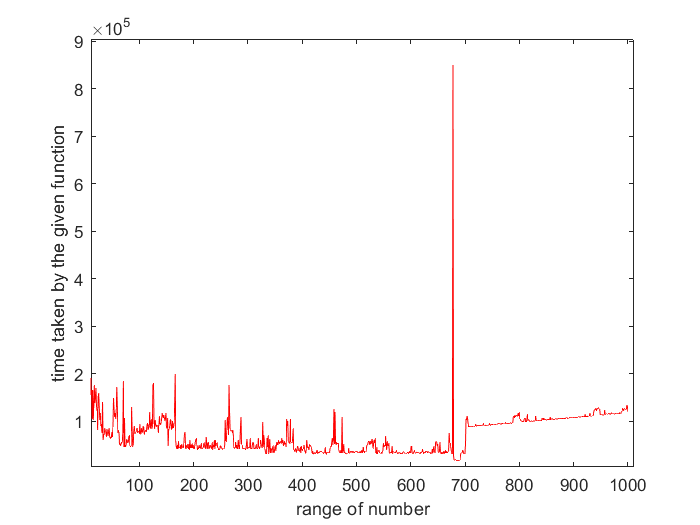
\includegraphics[scale=0.4]{multiplenew.png}
\caption{Figure: Graph showing the experimental analysis}\\
\end{figure}
Here as we can see , the given number if it is  prime or any such number which produces non-termination non-repeating decimal points or repeating decimals then the given number will produce peaks in graph .
\includegraphics[scale=0.4]{analysis.jpg}
\caption{Figure: Graph showing best case and worst case in between a given range of large numbers}\\
This graph shows particularly chosen such numbers and their analysis of time taken by the given functions.
\section{Discussion and Future Work}
Here we used string manipulation to generate reciprocal of any real number and bit manipulation to generate reciprocal of any integer . Both the method uses o($logn$) to solve the given problem . 
Another method could be to convert division problem into multiplication problem .One such method is to use Newton-Raphson method to find the multiplicative inverse without using division . Here let,\\ $f(x)$ $=$ $1/x-a$ , $f^\prime(x)$= $ -1/x^2$ \\
According to newton raphson method \\
$x_{n+1}$ = $x_n$ $-$ $f(x_n)/f^\prime(x_n)$
which yields ,\\ $x_{n+1}$ = $x_n(2-ax_n)$\\
Now , instead of division , multiplication of numbers should be performed .
Another method could be to use binary exponentiation method which also changes the algorithm from division to multiplication problem .
\section{Conclusion}
The given problem was solved using bit manipulation and iterative subtraction to perform division without using division operator to generate multiplicative inverse of the given number . Other method could be to solve using Newton Raphson method or through binary exponentiation method through multiplication .
\section{References}
\begin{enumerate}
\item IDAA432C (Design and Analysis of Algorithm) class lecture
\item Multiplicative inverse
\item Newton Raphson method
\item Introduction to Algorithms by Cormen
\end{enumerate}
\end{document}